% !TeX document-id = {d90bf12a-b9a7-4168-b165-ceabb359da2f}
% !TeX TXS-program:compile = txs:///pdflatex/[--shell-escape]
\documentclass{article}
\usepackage[a4paper,
paperwidth = 13cm, 
paperheight =5cm, 
textwidth = 13cm,
textheight = 5cm,
centering]{geometry}
\usepackage{tikz}
\usepackage{graphicx}
\usetikzlibrary{spy,
	positioning,
	arrows,
	arrows.meta,
	decorations.pathmorphing,
	calc,%
	decorations.pathmorphing,%
	decorations.markings,
	fadings,%
	shadings,%
	shapes,
	shapes.geometric,
	shapes.arrows,
	fit,
	plotmarks,}
\usetikzlibrary{arrows}

\usepackage{tikz-dimline}
\tikzset{
	myarrow/.style = {line width=0.9mm, draw=blue, -triangle 60, postaction={draw, line width=2mm, shorten >=4mm, -}}
}

\begin{document}

\begin{tikzpicture}[remember picture,overlay]
\node[anchor=south,xshift=3.8cm](ga1) at (current page.south) {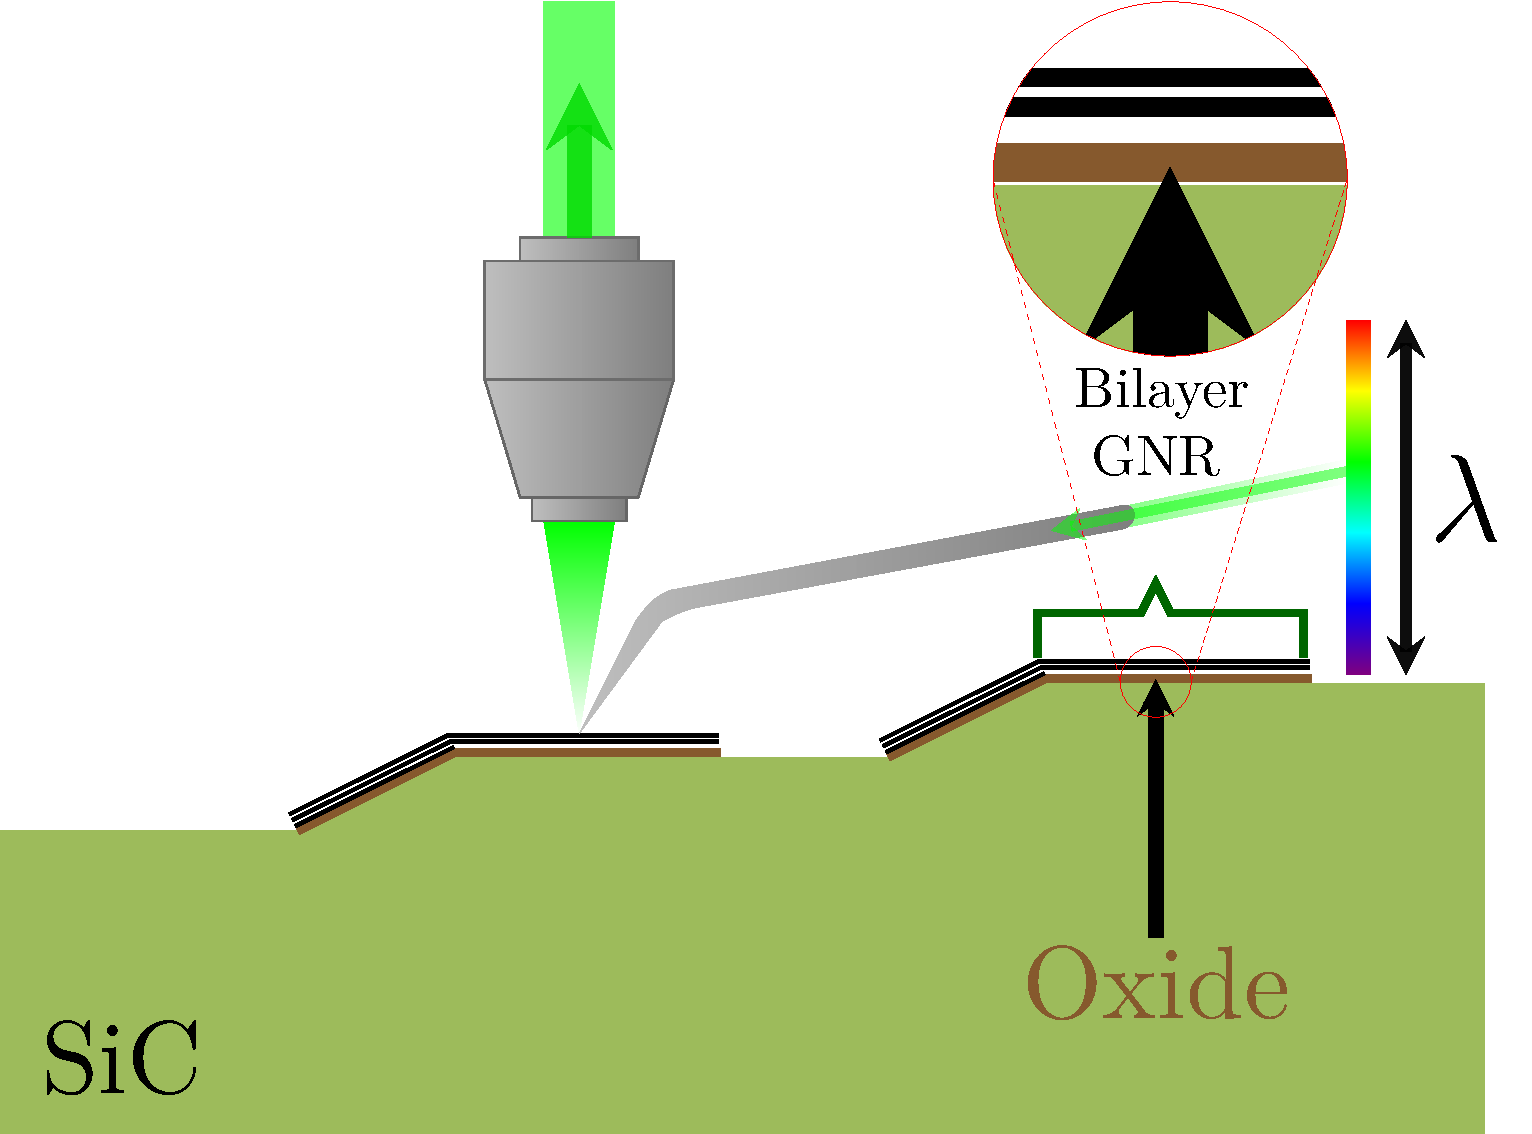
\includegraphics[scale=0.2]{GA-FINAL}};



\node[anchor=center,xshift=-2.8cm,yshift=20mm,draw,inner sep=0mm](nsom2) at (ga1.south west){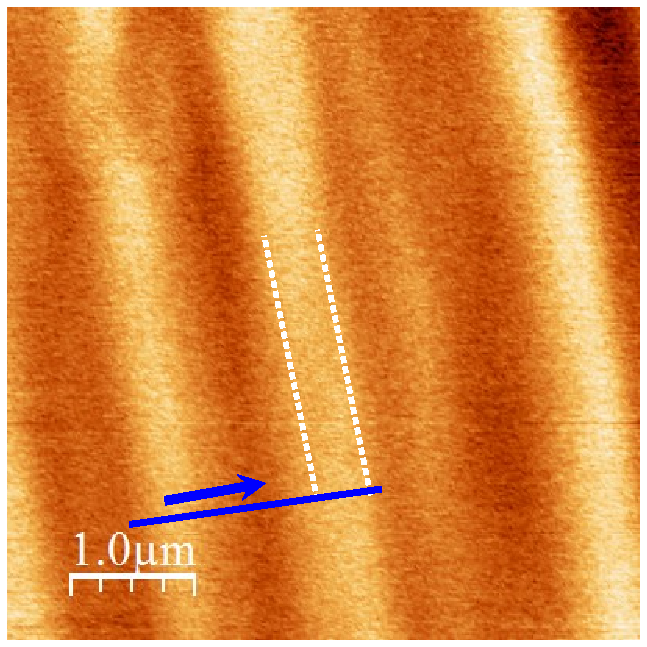
\includegraphics[scale=0.25]{GA-3}};
\node[anchor=south east,xshift=-2mm,yshift=-15mm](nsom3) at (nsom2.north west) {\includegraphics[scale=1.2]{spectra}};
\node[anchor=south west,xshift=-2mm,yshift=-15mm](nsom4) at (nsom2.north east) {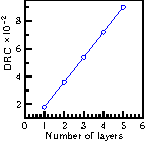
\includegraphics[scale=1.2]{DRC}};
%\draw[-{stealth},line width=10mm] (nsom2.center)--([xshift=80mm]nsom3.center);
\node[circle, minimum width=1mm,draw,anchor=center,line width=0.1mm](foc1) at ([xshift=-0.0mm,yshift=-1.5mm]nsom2.center){};
\draw[line width=0.1mm] ([xshift=-6.25mm,yshift=-5.5mm]ga1.center)--(foc1.south);
\draw[line width=0.1mm]  ([xshift=-6.25mm,yshift=-5.5mm]ga1.center)--(foc1.north);
%\draw[line width=3mm] ([xshift=15.8mm]nsom1.south west)--(foc1.north east);

\coordinate (n0) at (nsom2);  
\coordinate (n01) at (nsom3);  




%\node[draw, single arrow,red,
%minimum height=28mm, minimum width=1mm,
%single arrow head extend=1mm,
%fill=blue,
%opacity=0.1,
%xshift=-1mm,
%anchor=west, rotate=155] at (nsom2.center) {};

%\node[draw, 
%single arrow,
%red,
%minimum height=28mm, minimum width=1mm,
%single arrow head extend=1mm,
%yshift=5mm,
%fill=blue,
%opacity=0.1,
%anchor=west, rotate=0] at (nsom3.east) {};

\draw [myarrow,opacity=0.9] ([yshift=-1.27cm,xshift=-1.38cm]n0.south west)  to [out=180, in=270, looseness=1]  ([yshift=-1.2cm,xshift=-0.25cm]n01);

\draw [myarrow,opacity=0.9] ([yshift=5mm]nsom3.east)  to [out=0, in=180, looseness=0]  ([yshift=5mm]nsom4.west);

\end{tikzpicture}

\end{document}